\documentclass[a4paper]{article}

\usepackage{INTERSPEECH2021}

% Put the lab number of the corresponding exercise
\title{Language Modelling - Lab 4}
\name{Marco Prosperi (257857)}

\address{
  University of Trento}
\email{marco.prosperi@studenti.unitn.it}

\begin{document}

\maketitle

\section{Introduction}
The first part of the project aimed to improve the baseline RNN performance by incrementally adding 
features and dynamically adjusting hyperparameters (learning rate, hidden units,
embedding size). The model was trained on the Penn Treebank dataset, using perplexity
as the main evaluation metric. In the second part, advanced techniques \cite{merityRegOpt} were 
incorporated to further enhance the language model, including Weight Tying 
to reduce parameters, Variational Dropout (excluding DropConnect) for 
regularization, and Averaged Stochastic Gradient Descent (AvSGD) for better
optimization. These improvements aimed to enhance generalization and 
convergence while maintaining low perplexity (less than 250). 

\section{Implementation details}

\textbf{Part A: Incremental Architecture Enhancement.} Building upon the PyTorch implementation from the Lab Repository \cite{nlu-labs-unitn}, I systematically enhanced the baseline RNN model through architectural modifications and hyperparameter optimization. Starting with the RNN baseline that yielded high perplexity (173.22), I transitioned to an LSTM architecture, achieving significant improvement (137.31). Regularization through dropout layers further enhanced performance (123.14), while adopting the AdamW optimizer with weight decay produced the best Part A results (105.46). These incremental improvements demonstrated consistent performance gains and established the foundation for advanced techniques.

\textbf{Part B: Advanced Optimization Techniques.} I implemented three sophisticated methods from recent literature \cite{merityRegOpt}. Weight Tying reduced parameter count while improving generalization by sharing embedding and output layer weights. Variational Dropout \cite{gal2016theoreticallygroundedapplicationdropout} applied consistent dropout masks across temporal sequences, enhancing training stability for recurrent architectures compared to standard dropout.

\textbf{AvSGD Implementation Strategy.} Non-monotonically triggered AvSGD switches from SGD when performance plateaus, averaging parameter updates for improved convergence. Following the authors' recommendations, I implemented a patience-based trigger mechanism: when validation metrics stagnate over multiple epochs, AvSGD activation occurs with patience reset for early termination. Alternative triggering uses non-monotonic windows inspired by the Salesforce Research repository \cite{salesforce-repo}, monitoring validation loss deviations from observed minima.

\section{Results}
The experimental results are summarized in Table \ref{tab:results}. Part A demonstrated systematic performance improvements through architectural enhancements, progressing from RNN baseline (173.22) to LSTM with dropout and AdamW optimization (105.46). Figure \ref{fig:plot} illustrates the validation perplexity convergence for the best Part A configuration.

Part B achieved further optimization through advanced techniques. The final model with Weight Tying, Variational Dropout, and AvSGD reached 89.47 perplexity using learning rate 2 and 400 hidden/embedding units. Notably, StepLR scheduling (step size 5, gamma 0.75) proved crucial for convergence stability.

\textbf{AvSGD Optimization Dynamics.} An important observation during AvSGD triggering was temporary training loss increase, stemming from optimization dynamics shifts. When switching from SGD to averaged parameter updates, the model experiences trajectory disruption before stabilizing. The StepLR scheduler compounds this effect through conservative updates, requiring additional convergence steps. This temporary increase reflects transition toward flatter, more generalizable loss landscape minima, as shown in Figure \ref{fig:plot-avsdg}.

\begin{figure}[h!]
\centering
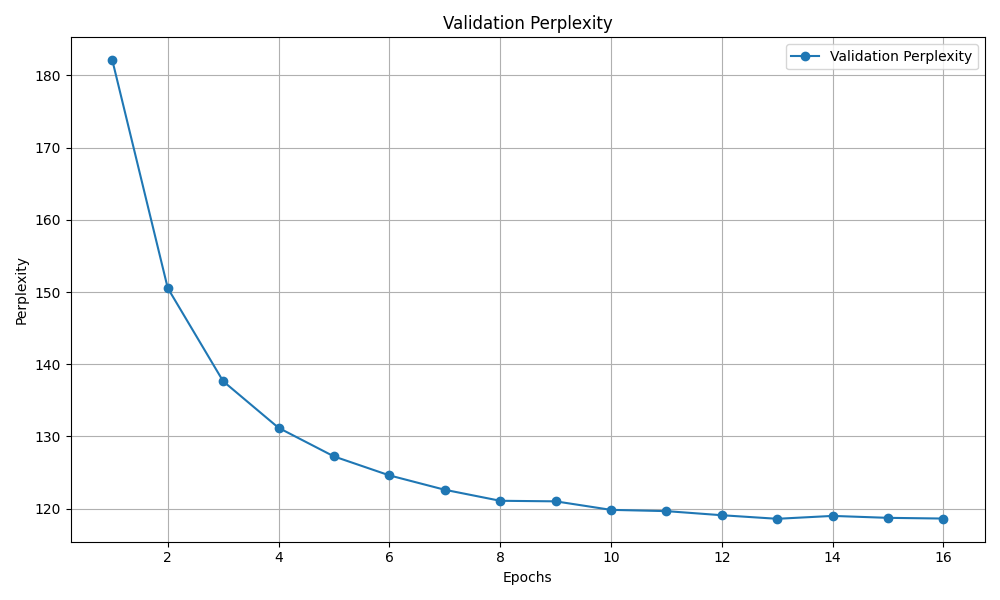
\includegraphics[width=0.8\linewidth]{images/part_A.png}
\caption{Validation perplexity of the LSTM model with dropout layers and AdamW.}
\label{fig:plot}
\end{figure}

\begin{figure}[h!]
\centering
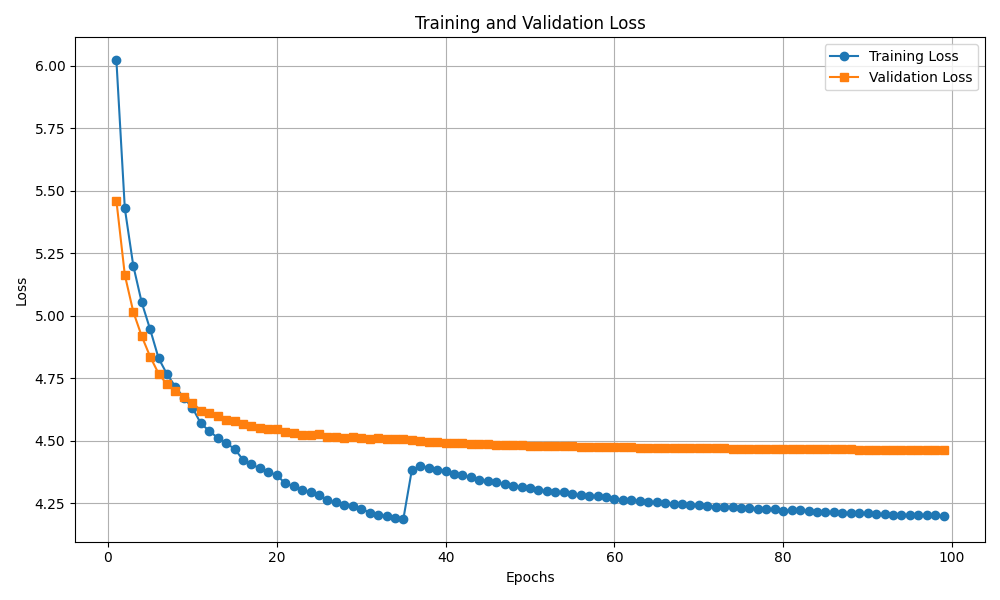
\includegraphics[width=0.8\linewidth]{images/part_A_avsdg.png}
\caption{Trigger point of AvSGD}
\label{fig:plot-avsdg}
\end{figure}

\begin{table}[h!]
  \centering
  \begin{tabular}{l p{1 cm} p{1 cm} p{1 cm} p{1 cm}}
      \midrule
      \textbf{Model} & \textbf{PPL} & \textbf{LR} & \textbf{Hidden} & \textbf{Emb} \\
      \midrule
      \multicolumn{5}{c}{\textbf{Part A}} \\
      RNN                     & 173.22 & 0.1    & 100 & 100 \\
      LSTM                    & 137.31 & 2      & 300 & 300 \\
      LSTM + Dropout Layers      & 123.14 & 2      & 300 & 300 \\
      LSTM + Dropout Layers + AdamW & 105.46 & 0.001 & 250 & 300 \\
      \midrule
      \multicolumn{5}{c}{\textbf{Part B}} \\
      \midrule
      LSTM + Weight Tying & 101.47 & 0.0015 & 400 & 400 \\
      LSTM + Weight Tying + Var Dropout & 96.68 & 0.01 & 400 & 400 \\
      LSTM + Weight Tying + Var Dropout + AvSDG & 89.47 & 2 & 400 & 400 \\
      \bottomrule
  \end{tabular}
  \caption{Perplexity and hyperparameters of the best models.}
  \label{tab:results}
\end{table}

\bibliographystyle{IEEEtran}

\bibliography{mybib}

\end{document}
